\batchmode
\documentclass[twoside]{book}

% Packages required by doxygen
\usepackage{fixltx2e}
\usepackage{calc}
\usepackage{doxygen}
\usepackage[export]{adjustbox} % also loads graphicx
\usepackage{graphicx}
\usepackage[utf8]{inputenc}
\usepackage{makeidx}
\usepackage{multicol}
\usepackage{multirow}
\PassOptionsToPackage{warn}{textcomp}
\usepackage{textcomp}
\usepackage[nointegrals]{wasysym}
\usepackage[table]{xcolor}

% Font selection
\usepackage[T1]{fontenc}
\usepackage[scaled=.90]{helvet}
\usepackage{courier}
\usepackage{amssymb}
\usepackage{sectsty}
\renewcommand{\familydefault}{\sfdefault}
\allsectionsfont{%
  \fontseries{bc}\selectfont%
  \color{darkgray}%
}
\renewcommand{\DoxyLabelFont}{%
  \fontseries{bc}\selectfont%
  \color{darkgray}%
}
\newcommand{\+}{\discretionary{\mbox{\scriptsize$\hookleftarrow$}}{}{}}

% Page & text layout
\usepackage{geometry}
\geometry{%
  a4paper,%
  top=2.5cm,%
  bottom=2.5cm,%
  left=2.5cm,%
  right=2.5cm%
}
\tolerance=750
\hfuzz=15pt
\hbadness=750
\setlength{\emergencystretch}{15pt}
\setlength{\parindent}{0cm}
\setlength{\parskip}{3ex plus 2ex minus 2ex}
\makeatletter
\renewcommand{\paragraph}{%
  \@startsection{paragraph}{4}{0ex}{-1.0ex}{1.0ex}{%
    \normalfont\normalsize\bfseries\SS@parafont%
  }%
}
\renewcommand{\subparagraph}{%
  \@startsection{subparagraph}{5}{0ex}{-1.0ex}{1.0ex}{%
    \normalfont\normalsize\bfseries\SS@subparafont%
  }%
}
\makeatother

% Headers & footers
\usepackage{fancyhdr}
\pagestyle{fancyplain}
\fancyhead[LE]{\fancyplain{}{\bfseries\thepage}}
\fancyhead[CE]{\fancyplain{}{}}
\fancyhead[RE]{\fancyplain{}{\bfseries\leftmark}}
\fancyhead[LO]{\fancyplain{}{\bfseries\rightmark}}
\fancyhead[CO]{\fancyplain{}{}}
\fancyhead[RO]{\fancyplain{}{\bfseries\thepage}}
\fancyfoot[LE]{\fancyplain{}{}}
\fancyfoot[CE]{\fancyplain{}{}}
\fancyfoot[RE]{\fancyplain{}{\bfseries\scriptsize Generated by Doxygen }}
\fancyfoot[LO]{\fancyplain{}{\bfseries\scriptsize Generated by Doxygen }}
\fancyfoot[CO]{\fancyplain{}{}}
\fancyfoot[RO]{\fancyplain{}{}}
\renewcommand{\footrulewidth}{0.4pt}
\renewcommand{\chaptermark}[1]{%
  \markboth{#1}{}%
}
\renewcommand{\sectionmark}[1]{%
  \markright{\thesection\ #1}%
}

% Indices & bibliography
\usepackage{natbib}
\usepackage[titles]{tocloft}
\setcounter{tocdepth}{3}
\setcounter{secnumdepth}{5}
\makeindex

% Hyperlinks (required, but should be loaded last)
\usepackage{ifpdf}
\ifpdf
  \usepackage[pdftex,pagebackref=true]{hyperref}
\else
  \usepackage[ps2pdf,pagebackref=true]{hyperref}
\fi
\hypersetup{%
  colorlinks=true,%
  linkcolor=blue,%
  citecolor=blue,%
  unicode%
}

% Custom commands
\newcommand{\clearemptydoublepage}{%
  \newpage{\pagestyle{empty}\cleardoublepage}%
}

\usepackage{caption}
\captionsetup{labelsep=space,justification=centering,font={bf},singlelinecheck=off,skip=4pt,position=top}

%===== C O N T E N T S =====

\begin{document}

% Titlepage & ToC
\hypersetup{pageanchor=false,
             bookmarksnumbered=true
            }
\pagenumbering{alph}
\pagenumbering{arabic}
\hypersetup{pageanchor=true}

%--- Begin generated contents ---
\chapter{Demo problem\+: Solution of the 2D linear wave equation}
\label{index}\hypertarget{index}{}\hypertarget{index_q}{}\section{A few quick questions...}\label{index_q}
Since {\ttfamily oomph-\/lib} is developed as open-\/source software, any evidence that the code is being downloaded and used is very helpful for us as it helps to justify our continued work on this project.

We would therefore be extremely grateful if you could provide the information requested in the form below. Pressing the \char`\"{}submit\char`\"{} button will get you to the actual download page.

{\bfseries Note\+:} 
\begin{DoxyItemize}
\item All information will be treated as confidential. 
\item If you provide your email address and check the appropriate box we will add you to our mailing list to inform you of upgrades and bug fixes to the code. Rest assured that the mailing list is {\bfseries very low volume} -- we have better things to do than to bombard you with email. 
\item If you still feel reluctant to provide any of the information requested, feel free to enter some dummy input. The form will check that {\bfseries some} information has been entered but entering your name as \char`\"{}\+Joe Cool\char`\"{} is perfectly acceptable -- this is to discourage people from not providing the information simply because they are too lazy to type... 
\end{DoxyItemize}



 







 

 \hypertarget{index_pdf}{}\section{P\+D\+F file}\label{index_pdf}
A \href{../latex/refman.pdf}{\tt pdf version} of this document is available. \end{document}

\chapter{Namespace Index}
\section{Namespace List}
Here is a list of all namespaces with brief descriptions\+:\begin{DoxyCompactList}
\item\contentsline{section}{\hyperlink{namespaceGlobal__Physical__Variables}{Global\+\_\+\+Physical\+\_\+\+Variables} \\*Global variables that represent physical properties }{\pageref{namespaceGlobal__Physical__Variables}}{}
\item\contentsline{section}{\hyperlink{namespaceoomph}{oomph} }{\pageref{namespaceoomph}}{}
\item\contentsline{section}{\hyperlink{namespacePhysical__Variables}{Physical\+\_\+\+Variables} \\*Namespace for the solution of 2D linear shell equation }{\pageref{namespacePhysical__Variables}}{}
\end{DoxyCompactList}

\chapter{Hierarchical Index}
\section{Class Hierarchy}
This inheritance list is sorted roughly, but not completely, alphabetically\+:\begin{DoxyCompactList}
\item Problem\begin{DoxyCompactList}
\item \contentsline{section}{Unstructured\+Solid\+Problem$<$ E\+L\+E\+M\+E\+NT $>$}{\pageref{classUnstructuredSolidProblem}}{}
\end{DoxyCompactList}
\end{DoxyCompactList}

\chapter{Class Index}
\section{Class List}
Here are the classes, structs, unions and interfaces with brief descriptions\+:\begin{DoxyCompactList}
\item\contentsline{section}{\hyperlink{classPMLProblem}{P\+M\+L\+Problem$<$ E\+L\+E\+M\+E\+N\+T $>$} }{\pageref{classPMLProblem}}{}
\item\contentsline{section}{\hyperlink{classGlobalParameters_1_1TestPMLMapping}{Global\+Parameters\+::\+Test\+P\+M\+L\+Mapping} }{\pageref{classGlobalParameters_1_1TestPMLMapping}}{}
\end{DoxyCompactList}

\chapter{File Index}
\section{File List}
Here is a list of all files with brief descriptions\+:\begin{DoxyCompactList}
\item\contentsline{section}{\hyperlink{jeffery__orbit_8cc}{jeffery\+\_\+orbit.\+cc} }{\pageref{jeffery__orbit_8cc}}{}
\item\contentsline{section}{\hyperlink{jeffery__orbit_8txt__doxygenified_8h}{jeffery\+\_\+orbit.\+txt\+\_\+doxygenified.\+h} }{\pageref{jeffery__orbit_8txt__doxygenified_8h}}{}
\item\contentsline{section}{\hyperlink{my__taylor__hood__elements_8h}{my\+\_\+taylor\+\_\+hood\+\_\+elements.\+h} }{\pageref{my__taylor__hood__elements_8h}}{}
\end{DoxyCompactList}

\chapter{Namespace Documentation}
\hypertarget{namespaceTanhSolnForLinearWave}{}\section{Tanh\+Soln\+For\+Linear\+Wave Namespace Reference}
\label{namespaceTanhSolnForLinearWave}\index{Tanh\+Soln\+For\+Linear\+Wave@{Tanh\+Soln\+For\+Linear\+Wave}}
\subsection*{Functions}
\begin{DoxyCompactItemize}
\item 
double \hyperlink{namespaceTanhSolnForLinearWave_aceea2935b2d3815ce72aae8c9de2b468}{exact\+\_\+u} (const double \&time, const Vector$<$ double $>$ \&x)
\begin{DoxyCompactList}\small\item\em Exact solution. \end{DoxyCompactList}\item 
double \hyperlink{namespaceTanhSolnForLinearWave_aa2081bd3d3d518a38497f664b0e498bc}{exact\+\_\+dudt} (const double \&time, const Vector$<$ double $>$ \&x)
\begin{DoxyCompactList}\small\item\em 1st time-\/deriv of exact solution \end{DoxyCompactList}\item 
double \hyperlink{namespaceTanhSolnForLinearWave_a63b7a0f5fd5d06cc2c0a43322a81fe43}{exact\+\_\+d2udt2} (const double \&time, const Vector$<$ double $>$ \&x)
\begin{DoxyCompactList}\small\item\em 2nd time-\/deriv of exact solution \end{DoxyCompactList}\item 
void \hyperlink{namespaceTanhSolnForLinearWave_a7dd7e9f155d19f871ba87d3fe41fd8e9}{get\+\_\+exact\+\_\+u} (const double \&time, const Vector$<$ double $>$ \&x, Vector$<$ double $>$ \&u)
\begin{DoxyCompactList}\small\item\em Exact solution as a vector. \end{DoxyCompactList}\item 
void \hyperlink{namespaceTanhSolnForLinearWave_a3bc9643b40e62283dc09f405ed17c805}{get\+\_\+source} (const double \&time, const Vector$<$ double $>$ \&x, double \&source)
\begin{DoxyCompactList}\small\item\em Source function to make it an exact solution. \end{DoxyCompactList}\item 
void \hyperlink{namespaceTanhSolnForLinearWave_af4c104781fc753f17614bcd8ac4fddc8}{get\+\_\+exact\+\_\+gradient} (const double \&time, const Vector$<$ double $>$ \&x, Vector$<$ double $>$ \&dudx)
\begin{DoxyCompactList}\small\item\em Gradient of exact solution. \end{DoxyCompactList}\item 
void \hyperlink{namespaceTanhSolnForLinearWave_a5a56ef7a715cb0b6e709f928d0f10592}{prescribed\+\_\+flux\+\_\+on\+\_\+fixed\+\_\+y\+\_\+boundary} (const double \&time, const Vector$<$ double $>$ \&x, double \&flux)
\begin{DoxyCompactList}\small\item\em Prescribed flux on a fixed y max boundary. \end{DoxyCompactList}\end{DoxyCompactItemize}
\subsection*{Variables}
\begin{DoxyCompactItemize}
\item 
double \hyperlink{namespaceTanhSolnForLinearWave_a48021142056bdea20e6432e360fd0314}{Alpha}
\begin{DoxyCompactList}\small\item\em Parameter for steepness of step. \end{DoxyCompactList}\item 
double \hyperlink{namespaceTanhSolnForLinearWave_a5242d421b567b803323bc127081351a6}{Phi}
\begin{DoxyCompactList}\small\item\em Orientation of step wave. \end{DoxyCompactList}\end{DoxyCompactItemize}


\subsection{Detailed Description}
Namespace for exact solution for Linear\+Wave equation with sharp step

Namespace for travelling wave solution for Linear\+Wave equation with sharp step 

\subsection{Function Documentation}
\mbox{\Hypertarget{namespaceTanhSolnForLinearWave_a63b7a0f5fd5d06cc2c0a43322a81fe43}\label{namespaceTanhSolnForLinearWave_a63b7a0f5fd5d06cc2c0a43322a81fe43}} 
\index{Tanh\+Soln\+For\+Linear\+Wave@{Tanh\+Soln\+For\+Linear\+Wave}!exact\+\_\+d2udt2@{exact\+\_\+d2udt2}}
\index{exact\+\_\+d2udt2@{exact\+\_\+d2udt2}!Tanh\+Soln\+For\+Linear\+Wave@{Tanh\+Soln\+For\+Linear\+Wave}}
\subsubsection{\texorpdfstring{exact\+\_\+d2udt2()}{exact\_d2udt2()}}
{\footnotesize\ttfamily double Tanh\+Soln\+For\+Linear\+Wave\+::exact\+\_\+d2udt2 (\begin{DoxyParamCaption}\item[{const double \&}]{time,  }\item[{const Vector$<$ double $>$ \&}]{x }\end{DoxyParamCaption})}



2nd time-\/deriv of exact solution 



Definition at line 77 of file two\+\_\+d\+\_\+linear\+\_\+wave.\+cc.



Referenced by Linear\+Wave\+Problem$<$ E\+L\+E\+M\+E\+N\+T, T\+I\+M\+E\+S\+T\+E\+P\+P\+E\+R $>$\+::actions\+\_\+before\+\_\+implicit\+\_\+timestep(), get\+\_\+exact\+\_\+u(), Linear\+Wave\+Problem$<$ E\+L\+E\+M\+E\+N\+T, T\+I\+M\+E\+S\+T\+E\+P\+P\+E\+R $>$\+::\+Linear\+Wave\+Problem(), and Linear\+Wave\+Problem$<$ E\+L\+E\+M\+E\+N\+T, T\+I\+M\+E\+S\+T\+E\+P\+P\+E\+R $>$\+::set\+\_\+initial\+\_\+condition().

\mbox{\Hypertarget{namespaceTanhSolnForLinearWave_aa2081bd3d3d518a38497f664b0e498bc}\label{namespaceTanhSolnForLinearWave_aa2081bd3d3d518a38497f664b0e498bc}} 
\index{Tanh\+Soln\+For\+Linear\+Wave@{Tanh\+Soln\+For\+Linear\+Wave}!exact\+\_\+dudt@{exact\+\_\+dudt}}
\index{exact\+\_\+dudt@{exact\+\_\+dudt}!Tanh\+Soln\+For\+Linear\+Wave@{Tanh\+Soln\+For\+Linear\+Wave}}
\subsubsection{\texorpdfstring{exact\+\_\+dudt()}{exact\_dudt()}}
{\footnotesize\ttfamily double Tanh\+Soln\+For\+Linear\+Wave\+::exact\+\_\+dudt (\begin{DoxyParamCaption}\item[{const double \&}]{time,  }\item[{const Vector$<$ double $>$ \&}]{x }\end{DoxyParamCaption})}



1st time-\/deriv of exact solution 



Definition at line 69 of file two\+\_\+d\+\_\+linear\+\_\+wave.\+cc.



Referenced by Linear\+Wave\+Problem$<$ E\+L\+E\+M\+E\+N\+T, T\+I\+M\+E\+S\+T\+E\+P\+P\+E\+R $>$\+::actions\+\_\+before\+\_\+implicit\+\_\+timestep(), get\+\_\+exact\+\_\+u(), Linear\+Wave\+Problem$<$ E\+L\+E\+M\+E\+N\+T, T\+I\+M\+E\+S\+T\+E\+P\+P\+E\+R $>$\+::\+Linear\+Wave\+Problem(), and Linear\+Wave\+Problem$<$ E\+L\+E\+M\+E\+N\+T, T\+I\+M\+E\+S\+T\+E\+P\+P\+E\+R $>$\+::set\+\_\+initial\+\_\+condition().

\mbox{\Hypertarget{namespaceTanhSolnForLinearWave_aceea2935b2d3815ce72aae8c9de2b468}\label{namespaceTanhSolnForLinearWave_aceea2935b2d3815ce72aae8c9de2b468}} 
\index{Tanh\+Soln\+For\+Linear\+Wave@{Tanh\+Soln\+For\+Linear\+Wave}!exact\+\_\+u@{exact\+\_\+u}}
\index{exact\+\_\+u@{exact\+\_\+u}!Tanh\+Soln\+For\+Linear\+Wave@{Tanh\+Soln\+For\+Linear\+Wave}}
\subsubsection{\texorpdfstring{exact\+\_\+u()}{exact\_u()}}
{\footnotesize\ttfamily double Tanh\+Soln\+For\+Linear\+Wave\+::exact\+\_\+u (\begin{DoxyParamCaption}\item[{const double \&}]{time,  }\item[{const Vector$<$ double $>$ \&}]{x }\end{DoxyParamCaption})}



Exact solution. 



Definition at line 62 of file two\+\_\+d\+\_\+linear\+\_\+wave.\+cc.



Referenced by Linear\+Wave\+Problem$<$ E\+L\+E\+M\+E\+N\+T, T\+I\+M\+E\+S\+T\+E\+P\+P\+E\+R $>$\+::actions\+\_\+before\+\_\+implicit\+\_\+timestep(), get\+\_\+exact\+\_\+u(), Linear\+Wave\+Problem$<$ E\+L\+E\+M\+E\+N\+T, T\+I\+M\+E\+S\+T\+E\+P\+P\+E\+R $>$\+::\+Linear\+Wave\+Problem(), and Linear\+Wave\+Problem$<$ E\+L\+E\+M\+E\+N\+T, T\+I\+M\+E\+S\+T\+E\+P\+P\+E\+R $>$\+::set\+\_\+initial\+\_\+condition().

\mbox{\Hypertarget{namespaceTanhSolnForLinearWave_af4c104781fc753f17614bcd8ac4fddc8}\label{namespaceTanhSolnForLinearWave_af4c104781fc753f17614bcd8ac4fddc8}} 
\index{Tanh\+Soln\+For\+Linear\+Wave@{Tanh\+Soln\+For\+Linear\+Wave}!get\+\_\+exact\+\_\+gradient@{get\+\_\+exact\+\_\+gradient}}
\index{get\+\_\+exact\+\_\+gradient@{get\+\_\+exact\+\_\+gradient}!Tanh\+Soln\+For\+Linear\+Wave@{Tanh\+Soln\+For\+Linear\+Wave}}
\subsubsection{\texorpdfstring{get\+\_\+exact\+\_\+gradient()}{get\_exact\_gradient()}}
{\footnotesize\ttfamily void Tanh\+Soln\+For\+Linear\+Wave\+::get\+\_\+exact\+\_\+gradient (\begin{DoxyParamCaption}\item[{const double \&}]{time,  }\item[{const Vector$<$ double $>$ \&}]{x,  }\item[{Vector$<$ double $>$ \&}]{dudx }\end{DoxyParamCaption})}



Gradient of exact solution. 



Definition at line 100 of file two\+\_\+d\+\_\+linear\+\_\+wave\+\_\+flux.\+cc.



Referenced by prescribed\+\_\+flux\+\_\+on\+\_\+fixed\+\_\+y\+\_\+boundary().

\mbox{\Hypertarget{namespaceTanhSolnForLinearWave_a7dd7e9f155d19f871ba87d3fe41fd8e9}\label{namespaceTanhSolnForLinearWave_a7dd7e9f155d19f871ba87d3fe41fd8e9}} 
\index{Tanh\+Soln\+For\+Linear\+Wave@{Tanh\+Soln\+For\+Linear\+Wave}!get\+\_\+exact\+\_\+u@{get\+\_\+exact\+\_\+u}}
\index{get\+\_\+exact\+\_\+u@{get\+\_\+exact\+\_\+u}!Tanh\+Soln\+For\+Linear\+Wave@{Tanh\+Soln\+For\+Linear\+Wave}}
\subsubsection{\texorpdfstring{get\+\_\+exact\+\_\+u()}{get\_exact\_u()}}
{\footnotesize\ttfamily void Tanh\+Soln\+For\+Linear\+Wave\+::get\+\_\+exact\+\_\+u (\begin{DoxyParamCaption}\item[{const double \&}]{time,  }\item[{const Vector$<$ double $>$ \&}]{x,  }\item[{Vector$<$ double $>$ \&}]{u }\end{DoxyParamCaption})}



Exact solution as a vector. 



Definition at line 86 of file two\+\_\+d\+\_\+linear\+\_\+wave.\+cc.



References exact\+\_\+d2udt2(), exact\+\_\+dudt(), and exact\+\_\+u().



Referenced by Linear\+Wave\+Problem$<$ E\+L\+E\+M\+E\+N\+T, T\+I\+M\+E\+S\+T\+E\+P\+P\+E\+R $>$\+::create\+\_\+flux\+\_\+elements(), and Linear\+Wave\+Problem$<$ E\+L\+E\+M\+E\+N\+T, T\+I\+M\+E\+S\+T\+E\+P\+P\+E\+R $>$\+::doc\+\_\+solution().

\mbox{\Hypertarget{namespaceTanhSolnForLinearWave_a3bc9643b40e62283dc09f405ed17c805}\label{namespaceTanhSolnForLinearWave_a3bc9643b40e62283dc09f405ed17c805}} 
\index{Tanh\+Soln\+For\+Linear\+Wave@{Tanh\+Soln\+For\+Linear\+Wave}!get\+\_\+source@{get\+\_\+source}}
\index{get\+\_\+source@{get\+\_\+source}!Tanh\+Soln\+For\+Linear\+Wave@{Tanh\+Soln\+For\+Linear\+Wave}}
\subsubsection{\texorpdfstring{get\+\_\+source()}{get\_source()}}
{\footnotesize\ttfamily void Tanh\+Soln\+For\+Linear\+Wave\+::get\+\_\+source (\begin{DoxyParamCaption}\item[{const double \&}]{time,  }\item[{const Vector$<$ double $>$ \&}]{x,  }\item[{double \&}]{source }\end{DoxyParamCaption})}



Source function to make it an exact solution. 



Definition at line 95 of file two\+\_\+d\+\_\+linear\+\_\+wave.\+cc.



Referenced by main().

\mbox{\Hypertarget{namespaceTanhSolnForLinearWave_a5a56ef7a715cb0b6e709f928d0f10592}\label{namespaceTanhSolnForLinearWave_a5a56ef7a715cb0b6e709f928d0f10592}} 
\index{Tanh\+Soln\+For\+Linear\+Wave@{Tanh\+Soln\+For\+Linear\+Wave}!prescribed\+\_\+flux\+\_\+on\+\_\+fixed\+\_\+y\+\_\+boundary@{prescribed\+\_\+flux\+\_\+on\+\_\+fixed\+\_\+y\+\_\+boundary}}
\index{prescribed\+\_\+flux\+\_\+on\+\_\+fixed\+\_\+y\+\_\+boundary@{prescribed\+\_\+flux\+\_\+on\+\_\+fixed\+\_\+y\+\_\+boundary}!Tanh\+Soln\+For\+Linear\+Wave@{Tanh\+Soln\+For\+Linear\+Wave}}
\subsubsection{\texorpdfstring{prescribed\+\_\+flux\+\_\+on\+\_\+fixed\+\_\+y\+\_\+boundary()}{prescribed\_flux\_on\_fixed\_y\_boundary()}}
{\footnotesize\ttfamily void Tanh\+Soln\+For\+Linear\+Wave\+::prescribed\+\_\+flux\+\_\+on\+\_\+fixed\+\_\+y\+\_\+boundary (\begin{DoxyParamCaption}\item[{const double \&}]{time,  }\item[{const Vector$<$ double $>$ \&}]{x,  }\item[{double \&}]{flux }\end{DoxyParamCaption})}



Prescribed flux on a fixed y max boundary. 



Definition at line 112 of file two\+\_\+d\+\_\+linear\+\_\+wave\+\_\+flux.\+cc.



References get\+\_\+exact\+\_\+gradient().



Referenced by Linear\+Wave\+Problem$<$ E\+L\+E\+M\+E\+N\+T, T\+I\+M\+E\+S\+T\+E\+P\+P\+E\+R $>$\+::\+Linear\+Wave\+Problem().



\subsection{Variable Documentation}
\mbox{\Hypertarget{namespaceTanhSolnForLinearWave_a48021142056bdea20e6432e360fd0314}\label{namespaceTanhSolnForLinearWave_a48021142056bdea20e6432e360fd0314}} 
\index{Tanh\+Soln\+For\+Linear\+Wave@{Tanh\+Soln\+For\+Linear\+Wave}!Alpha@{Alpha}}
\index{Alpha@{Alpha}!Tanh\+Soln\+For\+Linear\+Wave@{Tanh\+Soln\+For\+Linear\+Wave}}
\subsubsection{\texorpdfstring{Alpha}{Alpha}}
{\footnotesize\ttfamily double Tanh\+Soln\+For\+Linear\+Wave\+::\+Alpha}



Parameter for steepness of step. 



Definition at line 56 of file two\+\_\+d\+\_\+linear\+\_\+wave.\+cc.



Referenced by Linear\+Wave\+Problem$<$ E\+L\+E\+M\+E\+N\+T, T\+I\+M\+E\+S\+T\+E\+P\+P\+E\+R $>$\+::\+Linear\+Wave\+Problem().

\mbox{\Hypertarget{namespaceTanhSolnForLinearWave_a5242d421b567b803323bc127081351a6}\label{namespaceTanhSolnForLinearWave_a5242d421b567b803323bc127081351a6}} 
\index{Tanh\+Soln\+For\+Linear\+Wave@{Tanh\+Soln\+For\+Linear\+Wave}!Phi@{Phi}}
\index{Phi@{Phi}!Tanh\+Soln\+For\+Linear\+Wave@{Tanh\+Soln\+For\+Linear\+Wave}}
\subsubsection{\texorpdfstring{Phi}{Phi}}
{\footnotesize\ttfamily double Tanh\+Soln\+For\+Linear\+Wave\+::\+Phi}



Orientation of step wave. 



Definition at line 59 of file two\+\_\+d\+\_\+linear\+\_\+wave.\+cc.



Referenced by Linear\+Wave\+Problem$<$ E\+L\+E\+M\+E\+N\+T, T\+I\+M\+E\+S\+T\+E\+P\+P\+E\+R $>$\+::\+Linear\+Wave\+Problem().


\chapter{Class Documentation}
\hypertarget{classLinearWaveProblem}{}\section{Linear\+Wave\+Problem$<$ E\+L\+E\+M\+E\+NT, T\+I\+M\+E\+S\+T\+E\+P\+P\+ER $>$ Class Template Reference}
\label{classLinearWaveProblem}\index{Linear\+Wave\+Problem$<$ E\+L\+E\+M\+E\+N\+T, T\+I\+M\+E\+S\+T\+E\+P\+P\+E\+R $>$@{Linear\+Wave\+Problem$<$ E\+L\+E\+M\+E\+N\+T, T\+I\+M\+E\+S\+T\+E\+P\+P\+E\+R $>$}}


Linear\+Wave problem in rectanglular domain.  


Inheritance diagram for Linear\+Wave\+Problem$<$ E\+L\+E\+M\+E\+NT, T\+I\+M\+E\+S\+T\+E\+P\+P\+ER $>$\+:\begin{figure}[H]
\begin{center}
\leavevmode
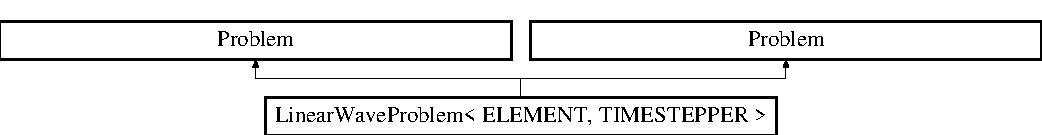
\includegraphics[height=1.812298cm]{classLinearWaveProblem}
\end{center}
\end{figure}
\subsection*{Public Member Functions}
\begin{DoxyCompactItemize}
\item 
\hyperlink{classLinearWaveProblem_a459a58b7afd588cfa78a5e1e98c3c41e}{Linear\+Wave\+Problem} (const unsigned \&nx, const unsigned \&ny, const bool \&impulsive\+\_\+start, Linear\+Wave\+Equations$<$ 2 $>$\+::Linear\+Wave\+Source\+Fct\+Pt source\+\_\+fct\+\_\+pt)
\begin{DoxyCompactList}\small\item\em Constructor\+: pass number of elements in x and y directions, bool indicating impulsive or \char`\"{}smooth\char`\"{} start, and pointer to source function. \end{DoxyCompactList}\item 
\hyperlink{classLinearWaveProblem_af1f3879114813b0acdfd2567c5c7b1e9}{$\sim$\+Linear\+Wave\+Problem} ()
\begin{DoxyCompactList}\small\item\em Destructor (empty) \end{DoxyCompactList}\item 
void \hyperlink{classLinearWaveProblem_a5b45c619af141b19162f990a95490e80}{actions\+\_\+after\+\_\+newton\+\_\+solve} ()
\begin{DoxyCompactList}\small\item\em Update the problem specs after solve (empty) \end{DoxyCompactList}\item 
void \hyperlink{classLinearWaveProblem_a66e87510f6fa8af693cede514cb7a62e}{actions\+\_\+before\+\_\+newton\+\_\+solve} ()
\begin{DoxyCompactList}\small\item\em Update the problem specs before solve (empty) \end{DoxyCompactList}\item 
void \hyperlink{classLinearWaveProblem_a521290f43f9aac37c9604e744fa71075}{actions\+\_\+after\+\_\+implicit\+\_\+timestep} ()
\begin{DoxyCompactList}\small\item\em Update the problem specs after solve (empty) \end{DoxyCompactList}\item 
void \hyperlink{classLinearWaveProblem_a39cfcb8ce06463ace1ac09fa43afa00a}{actions\+\_\+before\+\_\+implicit\+\_\+timestep} ()
\begin{DoxyCompactList}\small\item\em Update the problem specs before next timestep\+: Set time-\/dependent Dirchlet boundary from exact solution. \end{DoxyCompactList}\item 
void \hyperlink{classLinearWaveProblem_afb5d327791d8289a8a0a565afc8aee37}{set\+\_\+initial\+\_\+condition} ()
\begin{DoxyCompactList}\small\item\em Set initial condition (incl history values) \end{DoxyCompactList}\item 
void \hyperlink{classLinearWaveProblem_a6d9396a693be0479ece9ac1f14f9233a}{doc\+\_\+solution} (Doc\+Info \&doc\+\_\+info)
\begin{DoxyCompactList}\small\item\em Doc the solution. \end{DoxyCompactList}\item 
void \hyperlink{classLinearWaveProblem_a9993365201bfffcc04dd2034f0d3d391}{unsteady\+\_\+run} ()
\begin{DoxyCompactList}\small\item\em Do unsteady run. \end{DoxyCompactList}\item 
\hyperlink{classLinearWaveProblem_a8f49994bc293eee5946b79871ee78ea3}{Linear\+Wave\+Problem} (const unsigned \&nx, const unsigned \&ny, Linear\+Wave\+Equations$<$ 2 $>$\+::Linear\+Wave\+Source\+Fct\+Pt source\+\_\+fct\+\_\+pt)
\begin{DoxyCompactList}\small\item\em Constructor\+: pass number of elements in x and y directions and pointer to source function. \end{DoxyCompactList}\item 
\hyperlink{classLinearWaveProblem_af1f3879114813b0acdfd2567c5c7b1e9}{$\sim$\+Linear\+Wave\+Problem} ()
\begin{DoxyCompactList}\small\item\em Destructor (empty) \end{DoxyCompactList}\item 
void \hyperlink{classLinearWaveProblem_a5b45c619af141b19162f990a95490e80}{actions\+\_\+after\+\_\+newton\+\_\+solve} ()
\begin{DoxyCompactList}\small\item\em Update the problem specs after solve (empty) \end{DoxyCompactList}\item 
void \hyperlink{classLinearWaveProblem_a66e87510f6fa8af693cede514cb7a62e}{actions\+\_\+before\+\_\+newton\+\_\+solve} ()
\begin{DoxyCompactList}\small\item\em Update the problem specs before solve (empty) \end{DoxyCompactList}\item 
void \hyperlink{classLinearWaveProblem_a521290f43f9aac37c9604e744fa71075}{actions\+\_\+after\+\_\+implicit\+\_\+timestep} ()
\begin{DoxyCompactList}\small\item\em Update the problem specs after solve (empty) \end{DoxyCompactList}\item 
void \hyperlink{classLinearWaveProblem_a39cfcb8ce06463ace1ac09fa43afa00a}{actions\+\_\+before\+\_\+implicit\+\_\+timestep} ()
\begin{DoxyCompactList}\small\item\em Update the problem specs before next timestep\+: Set Dirchlet boundary conditions from exact solution. \end{DoxyCompactList}\item 
void \hyperlink{classLinearWaveProblem_afb5d327791d8289a8a0a565afc8aee37}{set\+\_\+initial\+\_\+condition} ()
\begin{DoxyCompactList}\small\item\em Set initial condition (incl history values) according to specified function. \end{DoxyCompactList}\item 
void \hyperlink{classLinearWaveProblem_a6d9396a693be0479ece9ac1f14f9233a}{doc\+\_\+solution} (Doc\+Info \&doc\+\_\+info)
\begin{DoxyCompactList}\small\item\em Doc the solution. \end{DoxyCompactList}\item 
void \hyperlink{classLinearWaveProblem_a9993365201bfffcc04dd2034f0d3d391}{unsteady\+\_\+run} ()
\begin{DoxyCompactList}\small\item\em Do unsteady run. \end{DoxyCompactList}\end{DoxyCompactItemize}
\subsection*{Private Member Functions}
\begin{DoxyCompactItemize}
\item 
void \hyperlink{classLinearWaveProblem_a2ea8935076615413cc864e127345b1c0}{create\+\_\+flux\+\_\+elements} (const unsigned \&b, Mesh $\ast$const \&bulk\+\_\+mesh\+\_\+pt, Mesh $\ast$const \&surface\+\_\+mesh\+\_\+pt)
\begin{DoxyCompactList}\small\item\em Create Linear\+Wave flux elements on boundary b of the Mesh pointed to by bulk\+\_\+mesh\+\_\+pt and add them to the Mesh object pointed to by surface\+\_\+mesh\+\_\+pt. \end{DoxyCompactList}\end{DoxyCompactItemize}
\subsection*{Private Attributes}
\begin{DoxyCompactItemize}
\item 
ofstream \hyperlink{classLinearWaveProblem_ac75d13211cfb08c7cfba0ea129711a09}{Trace\+\_\+file}
\item 
bool \hyperlink{classLinearWaveProblem_a296c67402f065a1a3776064492003670}{Impulsive\+\_\+start}
\item 
Rectangular\+Quad\+Mesh$<$ E\+L\+E\+M\+E\+NT $>$ $\ast$ \hyperlink{classLinearWaveProblem_aace6aa3bcf449d57976786ef776c0f5a}{Bulk\+\_\+mesh\+\_\+pt}
\begin{DoxyCompactList}\small\item\em Pointer to the \char`\"{}bulk\char`\"{} mesh. \end{DoxyCompactList}\item 
Mesh $\ast$ \hyperlink{classLinearWaveProblem_a286d4ca798729d03303b072bb704593f}{Surface\+\_\+mesh\+\_\+pt}
\begin{DoxyCompactList}\small\item\em Pointer to the \char`\"{}surface\char`\"{} mesh. \end{DoxyCompactList}\end{DoxyCompactItemize}


\subsection{Detailed Description}
\subsubsection*{template$<$class E\+L\+E\+M\+E\+NT, class T\+I\+M\+E\+S\+T\+E\+P\+P\+ER$>$\newline
class Linear\+Wave\+Problem$<$ E\+L\+E\+M\+E\+N\+T, T\+I\+M\+E\+S\+T\+E\+P\+P\+E\+R $>$}

Linear\+Wave problem in rectanglular domain. 

Linear\+Wave problem with flux boundary conditions in rectangle. 

Definition at line 112 of file two\+\_\+d\+\_\+linear\+\_\+wave.\+cc.



\subsection{Constructor \& Destructor Documentation}
\mbox{\Hypertarget{classLinearWaveProblem_a459a58b7afd588cfa78a5e1e98c3c41e}\label{classLinearWaveProblem_a459a58b7afd588cfa78a5e1e98c3c41e}} 
\index{Linear\+Wave\+Problem@{Linear\+Wave\+Problem}!Linear\+Wave\+Problem@{Linear\+Wave\+Problem}}
\index{Linear\+Wave\+Problem@{Linear\+Wave\+Problem}!Linear\+Wave\+Problem@{Linear\+Wave\+Problem}}
\subsubsection{\texorpdfstring{Linear\+Wave\+Problem()}{LinearWaveProblem()}\hspace{0.1cm}{\footnotesize\ttfamily [1/2]}}
{\footnotesize\ttfamily template$<$class E\+L\+E\+M\+E\+NT , class T\+I\+M\+E\+S\+T\+E\+P\+P\+ER $>$ \\
\hyperlink{classLinearWaveProblem}{Linear\+Wave\+Problem}$<$ E\+L\+E\+M\+E\+NT, T\+I\+M\+E\+S\+T\+E\+P\+P\+ER $>$\+::\hyperlink{classLinearWaveProblem}{Linear\+Wave\+Problem} (\begin{DoxyParamCaption}\item[{const unsigned \&}]{nx,  }\item[{const unsigned \&}]{ny,  }\item[{const bool \&}]{impulsive\+\_\+start,  }\item[{Linear\+Wave\+Equations$<$ 2 $>$\+::Linear\+Wave\+Source\+Fct\+Pt}]{source\+\_\+fct\+\_\+pt }\end{DoxyParamCaption})}



Constructor\+: pass number of elements in x and y directions, bool indicating impulsive or \char`\"{}smooth\char`\"{} start, and pointer to source function. 

Constructor for Linear\+Wave problem. 

Definition at line 216 of file two\+\_\+d\+\_\+linear\+\_\+wave.\+cc.



References Tanh\+Soln\+For\+Linear\+Wave\+::\+Alpha, and Tanh\+Soln\+For\+Linear\+Wave\+::\+Phi.

\mbox{\Hypertarget{classLinearWaveProblem_af1f3879114813b0acdfd2567c5c7b1e9}\label{classLinearWaveProblem_af1f3879114813b0acdfd2567c5c7b1e9}} 
\index{Linear\+Wave\+Problem@{Linear\+Wave\+Problem}!````~Linear\+Wave\+Problem@{$\sim$\+Linear\+Wave\+Problem}}
\index{````~Linear\+Wave\+Problem@{$\sim$\+Linear\+Wave\+Problem}!Linear\+Wave\+Problem@{Linear\+Wave\+Problem}}
\subsubsection{\texorpdfstring{$\sim$\+Linear\+Wave\+Problem()}{~LinearWaveProblem()}\hspace{0.1cm}{\footnotesize\ttfamily [1/2]}}
{\footnotesize\ttfamily template$<$class E\+L\+E\+M\+E\+NT, class T\+I\+M\+E\+S\+T\+E\+P\+P\+ER$>$ \\
\hyperlink{classLinearWaveProblem}{Linear\+Wave\+Problem}$<$ E\+L\+E\+M\+E\+NT, T\+I\+M\+E\+S\+T\+E\+P\+P\+ER $>$\+::$\sim$\hyperlink{classLinearWaveProblem}{Linear\+Wave\+Problem} (\begin{DoxyParamCaption}{ }\end{DoxyParamCaption})\hspace{0.3cm}{\ttfamily [inline]}}



Destructor (empty) 



Definition at line 125 of file two\+\_\+d\+\_\+linear\+\_\+wave.\+cc.

\mbox{\Hypertarget{classLinearWaveProblem_a8f49994bc293eee5946b79871ee78ea3}\label{classLinearWaveProblem_a8f49994bc293eee5946b79871ee78ea3}} 
\index{Linear\+Wave\+Problem@{Linear\+Wave\+Problem}!Linear\+Wave\+Problem@{Linear\+Wave\+Problem}}
\index{Linear\+Wave\+Problem@{Linear\+Wave\+Problem}!Linear\+Wave\+Problem@{Linear\+Wave\+Problem}}
\subsubsection{\texorpdfstring{Linear\+Wave\+Problem()}{LinearWaveProblem()}\hspace{0.1cm}{\footnotesize\ttfamily [2/2]}}
{\footnotesize\ttfamily template$<$class E\+L\+E\+M\+E\+NT , class T\+I\+M\+E\+S\+T\+E\+P\+P\+ER $>$ \\
\hyperlink{classLinearWaveProblem}{Linear\+Wave\+Problem}$<$ E\+L\+E\+M\+E\+NT, T\+I\+M\+E\+S\+T\+E\+P\+P\+ER $>$\+::\hyperlink{classLinearWaveProblem}{Linear\+Wave\+Problem} (\begin{DoxyParamCaption}\item[{const unsigned \&}]{nx,  }\item[{const unsigned \&}]{ny,  }\item[{Linear\+Wave\+Equations$<$ 2 $>$\+::Linear\+Wave\+Source\+Fct\+Pt}]{source\+\_\+fct\+\_\+pt }\end{DoxyParamCaption})}



Constructor\+: pass number of elements in x and y directions and pointer to source function. 

Constructor for Linear\+Wave problem. 

Definition at line 261 of file two\+\_\+d\+\_\+linear\+\_\+wave\+\_\+flux.\+cc.



References Tanh\+Soln\+For\+Linear\+Wave\+::\+Alpha, Linear\+Wave\+Problem$<$ E\+L\+E\+M\+E\+N\+T, T\+I\+M\+E\+S\+T\+E\+P\+P\+E\+R $>$\+::create\+\_\+flux\+\_\+elements(), Tanh\+Soln\+For\+Linear\+Wave\+::exact\+\_\+d2udt2(), Tanh\+Soln\+For\+Linear\+Wave\+::exact\+\_\+dudt(), Tanh\+Soln\+For\+Linear\+Wave\+::exact\+\_\+u(), Tanh\+Soln\+For\+Linear\+Wave\+::\+Phi, Tanh\+Soln\+For\+Linear\+Wave\+::prescribed\+\_\+flux\+\_\+on\+\_\+fixed\+\_\+y\+\_\+boundary(), and Linear\+Wave\+Problem$<$ E\+L\+E\+M\+E\+N\+T, T\+I\+M\+E\+S\+T\+E\+P\+P\+E\+R $>$\+::set\+\_\+initial\+\_\+condition().

\mbox{\Hypertarget{classLinearWaveProblem_af1f3879114813b0acdfd2567c5c7b1e9}\label{classLinearWaveProblem_af1f3879114813b0acdfd2567c5c7b1e9}} 
\index{Linear\+Wave\+Problem@{Linear\+Wave\+Problem}!````~Linear\+Wave\+Problem@{$\sim$\+Linear\+Wave\+Problem}}
\index{````~Linear\+Wave\+Problem@{$\sim$\+Linear\+Wave\+Problem}!Linear\+Wave\+Problem@{Linear\+Wave\+Problem}}
\subsubsection{\texorpdfstring{$\sim$\+Linear\+Wave\+Problem()}{~LinearWaveProblem()}\hspace{0.1cm}{\footnotesize\ttfamily [2/2]}}
{\footnotesize\ttfamily template$<$class E\+L\+E\+M\+E\+NT, class T\+I\+M\+E\+S\+T\+E\+P\+P\+ER$>$ \\
\hyperlink{classLinearWaveProblem}{Linear\+Wave\+Problem}$<$ E\+L\+E\+M\+E\+NT, T\+I\+M\+E\+S\+T\+E\+P\+P\+ER $>$\+::$\sim$\hyperlink{classLinearWaveProblem}{Linear\+Wave\+Problem} (\begin{DoxyParamCaption}{ }\end{DoxyParamCaption})\hspace{0.3cm}{\ttfamily [inline]}}



Destructor (empty) 



Definition at line 155 of file two\+\_\+d\+\_\+linear\+\_\+wave\+\_\+flux.\+cc.



\subsection{Member Function Documentation}
\mbox{\Hypertarget{classLinearWaveProblem_a521290f43f9aac37c9604e744fa71075}\label{classLinearWaveProblem_a521290f43f9aac37c9604e744fa71075}} 
\index{Linear\+Wave\+Problem@{Linear\+Wave\+Problem}!actions\+\_\+after\+\_\+implicit\+\_\+timestep@{actions\+\_\+after\+\_\+implicit\+\_\+timestep}}
\index{actions\+\_\+after\+\_\+implicit\+\_\+timestep@{actions\+\_\+after\+\_\+implicit\+\_\+timestep}!Linear\+Wave\+Problem@{Linear\+Wave\+Problem}}
\subsubsection{\texorpdfstring{actions\+\_\+after\+\_\+implicit\+\_\+timestep()}{actions\_after\_implicit\_timestep()}\hspace{0.1cm}{\footnotesize\ttfamily [1/2]}}
{\footnotesize\ttfamily template$<$class E\+L\+E\+M\+E\+NT, class T\+I\+M\+E\+S\+T\+E\+P\+P\+ER$>$ \\
void \hyperlink{classLinearWaveProblem}{Linear\+Wave\+Problem}$<$ E\+L\+E\+M\+E\+NT, T\+I\+M\+E\+S\+T\+E\+P\+P\+ER $>$\+::actions\+\_\+after\+\_\+implicit\+\_\+timestep (\begin{DoxyParamCaption}{ }\end{DoxyParamCaption})\hspace{0.3cm}{\ttfamily [inline]}}



Update the problem specs after solve (empty) 



Definition at line 134 of file two\+\_\+d\+\_\+linear\+\_\+wave.\+cc.

\mbox{\Hypertarget{classLinearWaveProblem_a521290f43f9aac37c9604e744fa71075}\label{classLinearWaveProblem_a521290f43f9aac37c9604e744fa71075}} 
\index{Linear\+Wave\+Problem@{Linear\+Wave\+Problem}!actions\+\_\+after\+\_\+implicit\+\_\+timestep@{actions\+\_\+after\+\_\+implicit\+\_\+timestep}}
\index{actions\+\_\+after\+\_\+implicit\+\_\+timestep@{actions\+\_\+after\+\_\+implicit\+\_\+timestep}!Linear\+Wave\+Problem@{Linear\+Wave\+Problem}}
\subsubsection{\texorpdfstring{actions\+\_\+after\+\_\+implicit\+\_\+timestep()}{actions\_after\_implicit\_timestep()}\hspace{0.1cm}{\footnotesize\ttfamily [2/2]}}
{\footnotesize\ttfamily template$<$class E\+L\+E\+M\+E\+NT, class T\+I\+M\+E\+S\+T\+E\+P\+P\+ER$>$ \\
void \hyperlink{classLinearWaveProblem}{Linear\+Wave\+Problem}$<$ E\+L\+E\+M\+E\+NT, T\+I\+M\+E\+S\+T\+E\+P\+P\+ER $>$\+::actions\+\_\+after\+\_\+implicit\+\_\+timestep (\begin{DoxyParamCaption}{ }\end{DoxyParamCaption})\hspace{0.3cm}{\ttfamily [inline]}}



Update the problem specs after solve (empty) 



Definition at line 164 of file two\+\_\+d\+\_\+linear\+\_\+wave\+\_\+flux.\+cc.

\mbox{\Hypertarget{classLinearWaveProblem_a5b45c619af141b19162f990a95490e80}\label{classLinearWaveProblem_a5b45c619af141b19162f990a95490e80}} 
\index{Linear\+Wave\+Problem@{Linear\+Wave\+Problem}!actions\+\_\+after\+\_\+newton\+\_\+solve@{actions\+\_\+after\+\_\+newton\+\_\+solve}}
\index{actions\+\_\+after\+\_\+newton\+\_\+solve@{actions\+\_\+after\+\_\+newton\+\_\+solve}!Linear\+Wave\+Problem@{Linear\+Wave\+Problem}}
\subsubsection{\texorpdfstring{actions\+\_\+after\+\_\+newton\+\_\+solve()}{actions\_after\_newton\_solve()}\hspace{0.1cm}{\footnotesize\ttfamily [1/2]}}
{\footnotesize\ttfamily template$<$class E\+L\+E\+M\+E\+NT, class T\+I\+M\+E\+S\+T\+E\+P\+P\+ER$>$ \\
void \hyperlink{classLinearWaveProblem}{Linear\+Wave\+Problem}$<$ E\+L\+E\+M\+E\+NT, T\+I\+M\+E\+S\+T\+E\+P\+P\+ER $>$\+::actions\+\_\+after\+\_\+newton\+\_\+solve (\begin{DoxyParamCaption}{ }\end{DoxyParamCaption})\hspace{0.3cm}{\ttfamily [inline]}}



Update the problem specs after solve (empty) 



Definition at line 128 of file two\+\_\+d\+\_\+linear\+\_\+wave.\+cc.

\mbox{\Hypertarget{classLinearWaveProblem_a5b45c619af141b19162f990a95490e80}\label{classLinearWaveProblem_a5b45c619af141b19162f990a95490e80}} 
\index{Linear\+Wave\+Problem@{Linear\+Wave\+Problem}!actions\+\_\+after\+\_\+newton\+\_\+solve@{actions\+\_\+after\+\_\+newton\+\_\+solve}}
\index{actions\+\_\+after\+\_\+newton\+\_\+solve@{actions\+\_\+after\+\_\+newton\+\_\+solve}!Linear\+Wave\+Problem@{Linear\+Wave\+Problem}}
\subsubsection{\texorpdfstring{actions\+\_\+after\+\_\+newton\+\_\+solve()}{actions\_after\_newton\_solve()}\hspace{0.1cm}{\footnotesize\ttfamily [2/2]}}
{\footnotesize\ttfamily template$<$class E\+L\+E\+M\+E\+NT, class T\+I\+M\+E\+S\+T\+E\+P\+P\+ER$>$ \\
void \hyperlink{classLinearWaveProblem}{Linear\+Wave\+Problem}$<$ E\+L\+E\+M\+E\+NT, T\+I\+M\+E\+S\+T\+E\+P\+P\+ER $>$\+::actions\+\_\+after\+\_\+newton\+\_\+solve (\begin{DoxyParamCaption}{ }\end{DoxyParamCaption})\hspace{0.3cm}{\ttfamily [inline]}}



Update the problem specs after solve (empty) 



Definition at line 158 of file two\+\_\+d\+\_\+linear\+\_\+wave\+\_\+flux.\+cc.

\mbox{\Hypertarget{classLinearWaveProblem_a39cfcb8ce06463ace1ac09fa43afa00a}\label{classLinearWaveProblem_a39cfcb8ce06463ace1ac09fa43afa00a}} 
\index{Linear\+Wave\+Problem@{Linear\+Wave\+Problem}!actions\+\_\+before\+\_\+implicit\+\_\+timestep@{actions\+\_\+before\+\_\+implicit\+\_\+timestep}}
\index{actions\+\_\+before\+\_\+implicit\+\_\+timestep@{actions\+\_\+before\+\_\+implicit\+\_\+timestep}!Linear\+Wave\+Problem@{Linear\+Wave\+Problem}}
\subsubsection{\texorpdfstring{actions\+\_\+before\+\_\+implicit\+\_\+timestep()}{actions\_before\_implicit\_timestep()}\hspace{0.1cm}{\footnotesize\ttfamily [1/2]}}
{\footnotesize\ttfamily template$<$class E\+L\+E\+M\+E\+NT, class T\+I\+M\+E\+S\+T\+E\+P\+P\+ER$>$ \\
void \hyperlink{classLinearWaveProblem}{Linear\+Wave\+Problem}$<$ E\+L\+E\+M\+E\+NT, T\+I\+M\+E\+S\+T\+E\+P\+P\+ER $>$\+::actions\+\_\+before\+\_\+implicit\+\_\+timestep (\begin{DoxyParamCaption}{ }\end{DoxyParamCaption})\hspace{0.3cm}{\ttfamily [inline]}}



Update the problem specs before next timestep\+: Set time-\/dependent Dirchlet boundary from exact solution. 



Definition at line 138 of file two\+\_\+d\+\_\+linear\+\_\+wave.\+cc.



References Tanh\+Soln\+For\+Linear\+Wave\+::exact\+\_\+d2udt2(), Tanh\+Soln\+For\+Linear\+Wave\+::exact\+\_\+dudt(), and Tanh\+Soln\+For\+Linear\+Wave\+::exact\+\_\+u().

\mbox{\Hypertarget{classLinearWaveProblem_a39cfcb8ce06463ace1ac09fa43afa00a}\label{classLinearWaveProblem_a39cfcb8ce06463ace1ac09fa43afa00a}} 
\index{Linear\+Wave\+Problem@{Linear\+Wave\+Problem}!actions\+\_\+before\+\_\+implicit\+\_\+timestep@{actions\+\_\+before\+\_\+implicit\+\_\+timestep}}
\index{actions\+\_\+before\+\_\+implicit\+\_\+timestep@{actions\+\_\+before\+\_\+implicit\+\_\+timestep}!Linear\+Wave\+Problem@{Linear\+Wave\+Problem}}
\subsubsection{\texorpdfstring{actions\+\_\+before\+\_\+implicit\+\_\+timestep()}{actions\_before\_implicit\_timestep()}\hspace{0.1cm}{\footnotesize\ttfamily [2/2]}}
{\footnotesize\ttfamily template$<$class E\+L\+E\+M\+E\+NT, class T\+I\+M\+E\+S\+T\+E\+P\+P\+ER$>$ \\
void \hyperlink{classLinearWaveProblem}{Linear\+Wave\+Problem}$<$ E\+L\+E\+M\+E\+NT, T\+I\+M\+E\+S\+T\+E\+P\+P\+ER $>$\+::actions\+\_\+before\+\_\+implicit\+\_\+timestep (\begin{DoxyParamCaption}{ }\end{DoxyParamCaption})\hspace{0.3cm}{\ttfamily [inline]}}



Update the problem specs before next timestep\+: Set Dirchlet boundary conditions from exact solution. 



Definition at line 168 of file two\+\_\+d\+\_\+linear\+\_\+wave\+\_\+flux.\+cc.



References Tanh\+Soln\+For\+Linear\+Wave\+::exact\+\_\+d2udt2(), Tanh\+Soln\+For\+Linear\+Wave\+::exact\+\_\+dudt(), and Tanh\+Soln\+For\+Linear\+Wave\+::exact\+\_\+u().

\mbox{\Hypertarget{classLinearWaveProblem_a66e87510f6fa8af693cede514cb7a62e}\label{classLinearWaveProblem_a66e87510f6fa8af693cede514cb7a62e}} 
\index{Linear\+Wave\+Problem@{Linear\+Wave\+Problem}!actions\+\_\+before\+\_\+newton\+\_\+solve@{actions\+\_\+before\+\_\+newton\+\_\+solve}}
\index{actions\+\_\+before\+\_\+newton\+\_\+solve@{actions\+\_\+before\+\_\+newton\+\_\+solve}!Linear\+Wave\+Problem@{Linear\+Wave\+Problem}}
\subsubsection{\texorpdfstring{actions\+\_\+before\+\_\+newton\+\_\+solve()}{actions\_before\_newton\_solve()}\hspace{0.1cm}{\footnotesize\ttfamily [1/2]}}
{\footnotesize\ttfamily template$<$class E\+L\+E\+M\+E\+NT, class T\+I\+M\+E\+S\+T\+E\+P\+P\+ER$>$ \\
void \hyperlink{classLinearWaveProblem}{Linear\+Wave\+Problem}$<$ E\+L\+E\+M\+E\+NT, T\+I\+M\+E\+S\+T\+E\+P\+P\+ER $>$\+::actions\+\_\+before\+\_\+newton\+\_\+solve (\begin{DoxyParamCaption}{ }\end{DoxyParamCaption})\hspace{0.3cm}{\ttfamily [inline]}}



Update the problem specs before solve (empty) 



Definition at line 131 of file two\+\_\+d\+\_\+linear\+\_\+wave.\+cc.

\mbox{\Hypertarget{classLinearWaveProblem_a66e87510f6fa8af693cede514cb7a62e}\label{classLinearWaveProblem_a66e87510f6fa8af693cede514cb7a62e}} 
\index{Linear\+Wave\+Problem@{Linear\+Wave\+Problem}!actions\+\_\+before\+\_\+newton\+\_\+solve@{actions\+\_\+before\+\_\+newton\+\_\+solve}}
\index{actions\+\_\+before\+\_\+newton\+\_\+solve@{actions\+\_\+before\+\_\+newton\+\_\+solve}!Linear\+Wave\+Problem@{Linear\+Wave\+Problem}}
\subsubsection{\texorpdfstring{actions\+\_\+before\+\_\+newton\+\_\+solve()}{actions\_before\_newton\_solve()}\hspace{0.1cm}{\footnotesize\ttfamily [2/2]}}
{\footnotesize\ttfamily template$<$class E\+L\+E\+M\+E\+NT, class T\+I\+M\+E\+S\+T\+E\+P\+P\+ER$>$ \\
void \hyperlink{classLinearWaveProblem}{Linear\+Wave\+Problem}$<$ E\+L\+E\+M\+E\+NT, T\+I\+M\+E\+S\+T\+E\+P\+P\+ER $>$\+::actions\+\_\+before\+\_\+newton\+\_\+solve (\begin{DoxyParamCaption}{ }\end{DoxyParamCaption})\hspace{0.3cm}{\ttfamily [inline]}}



Update the problem specs before solve (empty) 



Definition at line 161 of file two\+\_\+d\+\_\+linear\+\_\+wave\+\_\+flux.\+cc.

\mbox{\Hypertarget{classLinearWaveProblem_a2ea8935076615413cc864e127345b1c0}\label{classLinearWaveProblem_a2ea8935076615413cc864e127345b1c0}} 
\index{Linear\+Wave\+Problem@{Linear\+Wave\+Problem}!create\+\_\+flux\+\_\+elements@{create\+\_\+flux\+\_\+elements}}
\index{create\+\_\+flux\+\_\+elements@{create\+\_\+flux\+\_\+elements}!Linear\+Wave\+Problem@{Linear\+Wave\+Problem}}
\subsubsection{\texorpdfstring{create\+\_\+flux\+\_\+elements()}{create\_flux\_elements()}}
{\footnotesize\ttfamily template$<$class E\+L\+E\+M\+E\+NT , class T\+I\+M\+E\+S\+T\+E\+P\+P\+ER $>$ \\
void \hyperlink{classLinearWaveProblem}{Linear\+Wave\+Problem}$<$ E\+L\+E\+M\+E\+NT, T\+I\+M\+E\+S\+T\+E\+P\+P\+ER $>$\+::create\+\_\+flux\+\_\+elements (\begin{DoxyParamCaption}\item[{const unsigned \&}]{b,  }\item[{Mesh $\ast$const \&}]{bulk\+\_\+mesh\+\_\+pt,  }\item[{Mesh $\ast$const \&}]{surface\+\_\+mesh\+\_\+pt }\end{DoxyParamCaption})\hspace{0.3cm}{\ttfamily [private]}}



Create Linear\+Wave flux elements on boundary b of the Mesh pointed to by bulk\+\_\+mesh\+\_\+pt and add them to the Mesh object pointed to by surface\+\_\+mesh\+\_\+pt. 

Create Linear\+Wave Flux Elements on the b-\/th boundary of the Mesh object pointed to by bulk\+\_\+mesh\+\_\+pt and add the elements to the Mesh object pointed to by surface\+\_\+mesh\+\_\+pt. 

Definition at line 427 of file two\+\_\+d\+\_\+linear\+\_\+wave\+\_\+flux.\+cc.



References Linear\+Wave\+Problem$<$ E\+L\+E\+M\+E\+N\+T, T\+I\+M\+E\+S\+T\+E\+P\+P\+E\+R $>$\+::doc\+\_\+solution(), Tanh\+Soln\+For\+Linear\+Wave\+::get\+\_\+exact\+\_\+u(), and Linear\+Wave\+Problem$<$ E\+L\+E\+M\+E\+N\+T, T\+I\+M\+E\+S\+T\+E\+P\+P\+E\+R $>$\+::unsteady\+\_\+run().



Referenced by Linear\+Wave\+Problem$<$ E\+L\+E\+M\+E\+N\+T, T\+I\+M\+E\+S\+T\+E\+P\+P\+E\+R $>$\+::\+Linear\+Wave\+Problem().

\mbox{\Hypertarget{classLinearWaveProblem_a6d9396a693be0479ece9ac1f14f9233a}\label{classLinearWaveProblem_a6d9396a693be0479ece9ac1f14f9233a}} 
\index{Linear\+Wave\+Problem@{Linear\+Wave\+Problem}!doc\+\_\+solution@{doc\+\_\+solution}}
\index{doc\+\_\+solution@{doc\+\_\+solution}!Linear\+Wave\+Problem@{Linear\+Wave\+Problem}}
\subsubsection{\texorpdfstring{doc\+\_\+solution()}{doc\_solution()}\hspace{0.1cm}{\footnotesize\ttfamily [1/2]}}
{\footnotesize\ttfamily template$<$class E\+L\+E\+M\+E\+NT , class T\+I\+M\+E\+S\+T\+E\+P\+P\+ER $>$ \\
void \hyperlink{classLinearWaveProblem}{Linear\+Wave\+Problem}$<$ E\+L\+E\+M\+E\+NT, T\+I\+M\+E\+S\+T\+E\+P\+P\+ER $>$\+::doc\+\_\+solution (\begin{DoxyParamCaption}\item[{Doc\+Info \&}]{doc\+\_\+info }\end{DoxyParamCaption})}



Doc the solution. 



Definition at line 408 of file two\+\_\+d\+\_\+linear\+\_\+wave.\+cc.



References Tanh\+Soln\+For\+Linear\+Wave\+::get\+\_\+exact\+\_\+u(), and Linear\+Wave\+Problem$<$ E\+L\+E\+M\+E\+N\+T, T\+I\+M\+E\+S\+T\+E\+P\+P\+E\+R $>$\+::\+Trace\+\_\+file.



Referenced by Linear\+Wave\+Problem$<$ E\+L\+E\+M\+E\+N\+T, T\+I\+M\+E\+S\+T\+E\+P\+P\+E\+R $>$\+::create\+\_\+flux\+\_\+elements(), and Linear\+Wave\+Problem$<$ E\+L\+E\+M\+E\+N\+T, T\+I\+M\+E\+S\+T\+E\+P\+P\+E\+R $>$\+::unsteady\+\_\+run().

\mbox{\Hypertarget{classLinearWaveProblem_a6d9396a693be0479ece9ac1f14f9233a}\label{classLinearWaveProblem_a6d9396a693be0479ece9ac1f14f9233a}} 
\index{Linear\+Wave\+Problem@{Linear\+Wave\+Problem}!doc\+\_\+solution@{doc\+\_\+solution}}
\index{doc\+\_\+solution@{doc\+\_\+solution}!Linear\+Wave\+Problem@{Linear\+Wave\+Problem}}
\subsubsection{\texorpdfstring{doc\+\_\+solution()}{doc\_solution()}\hspace{0.1cm}{\footnotesize\ttfamily [2/2]}}
{\footnotesize\ttfamily template$<$class E\+L\+E\+M\+E\+NT, class T\+I\+M\+E\+S\+T\+E\+P\+P\+ER$>$ \\
void \hyperlink{classLinearWaveProblem}{Linear\+Wave\+Problem}$<$ E\+L\+E\+M\+E\+NT, T\+I\+M\+E\+S\+T\+E\+P\+P\+ER $>$\+::doc\+\_\+solution (\begin{DoxyParamCaption}\item[{Doc\+Info \&}]{doc\+\_\+info }\end{DoxyParamCaption})}



Doc the solution. 

\mbox{\Hypertarget{classLinearWaveProblem_afb5d327791d8289a8a0a565afc8aee37}\label{classLinearWaveProblem_afb5d327791d8289a8a0a565afc8aee37}} 
\index{Linear\+Wave\+Problem@{Linear\+Wave\+Problem}!set\+\_\+initial\+\_\+condition@{set\+\_\+initial\+\_\+condition}}
\index{set\+\_\+initial\+\_\+condition@{set\+\_\+initial\+\_\+condition}!Linear\+Wave\+Problem@{Linear\+Wave\+Problem}}
\subsubsection{\texorpdfstring{set\+\_\+initial\+\_\+condition()}{set\_initial\_condition()}\hspace{0.1cm}{\footnotesize\ttfamily [1/2]}}
{\footnotesize\ttfamily template$<$class E\+L\+E\+M\+E\+NT , class T\+I\+M\+E\+S\+T\+E\+P\+P\+ER $>$ \\
void \hyperlink{classLinearWaveProblem}{Linear\+Wave\+Problem}$<$ E\+L\+E\+M\+E\+NT, T\+I\+M\+E\+S\+T\+E\+P\+P\+ER $>$\+::set\+\_\+initial\+\_\+condition (\begin{DoxyParamCaption}{ }\end{DoxyParamCaption})}



Set initial condition (incl history values) 

Set initial condition. 

Definition at line 293 of file two\+\_\+d\+\_\+linear\+\_\+wave.\+cc.



References Tanh\+Soln\+For\+Linear\+Wave\+::exact\+\_\+d2udt2(), Tanh\+Soln\+For\+Linear\+Wave\+::exact\+\_\+dudt(), Tanh\+Soln\+For\+Linear\+Wave\+::exact\+\_\+u(), and Linear\+Wave\+Problem$<$ E\+L\+E\+M\+E\+N\+T, T\+I\+M\+E\+S\+T\+E\+P\+P\+E\+R $>$\+::\+Impulsive\+\_\+start.



Referenced by Linear\+Wave\+Problem$<$ E\+L\+E\+M\+E\+N\+T, T\+I\+M\+E\+S\+T\+E\+P\+P\+E\+R $>$\+::\+Linear\+Wave\+Problem(), and Linear\+Wave\+Problem$<$ E\+L\+E\+M\+E\+N\+T, T\+I\+M\+E\+S\+T\+E\+P\+P\+E\+R $>$\+::unsteady\+\_\+run().

\mbox{\Hypertarget{classLinearWaveProblem_afb5d327791d8289a8a0a565afc8aee37}\label{classLinearWaveProblem_afb5d327791d8289a8a0a565afc8aee37}} 
\index{Linear\+Wave\+Problem@{Linear\+Wave\+Problem}!set\+\_\+initial\+\_\+condition@{set\+\_\+initial\+\_\+condition}}
\index{set\+\_\+initial\+\_\+condition@{set\+\_\+initial\+\_\+condition}!Linear\+Wave\+Problem@{Linear\+Wave\+Problem}}
\subsubsection{\texorpdfstring{set\+\_\+initial\+\_\+condition()}{set\_initial\_condition()}\hspace{0.1cm}{\footnotesize\ttfamily [2/2]}}
{\footnotesize\ttfamily template$<$class E\+L\+E\+M\+E\+NT, class T\+I\+M\+E\+S\+T\+E\+P\+P\+ER$>$ \\
void \hyperlink{classLinearWaveProblem}{Linear\+Wave\+Problem}$<$ E\+L\+E\+M\+E\+NT, T\+I\+M\+E\+S\+T\+E\+P\+P\+ER $>$\+::set\+\_\+initial\+\_\+condition (\begin{DoxyParamCaption}{ }\end{DoxyParamCaption})}



Set initial condition (incl history values) according to specified function. 

\mbox{\Hypertarget{classLinearWaveProblem_a9993365201bfffcc04dd2034f0d3d391}\label{classLinearWaveProblem_a9993365201bfffcc04dd2034f0d3d391}} 
\index{Linear\+Wave\+Problem@{Linear\+Wave\+Problem}!unsteady\+\_\+run@{unsteady\+\_\+run}}
\index{unsteady\+\_\+run@{unsteady\+\_\+run}!Linear\+Wave\+Problem@{Linear\+Wave\+Problem}}
\subsubsection{\texorpdfstring{unsteady\+\_\+run()}{unsteady\_run()}\hspace{0.1cm}{\footnotesize\ttfamily [1/2]}}
{\footnotesize\ttfamily template$<$class E\+L\+E\+M\+E\+NT , class T\+I\+M\+E\+S\+T\+E\+P\+P\+ER $>$ \\
void \hyperlink{classLinearWaveProblem}{Linear\+Wave\+Problem}$<$ E\+L\+E\+M\+E\+NT, T\+I\+M\+E\+S\+T\+E\+P\+P\+ER $>$\+::unsteady\+\_\+run (\begin{DoxyParamCaption}{ }\end{DoxyParamCaption})}



Do unsteady run. 

Perform run up to specified time.

Unsteady run. 

Definition at line 476 of file two\+\_\+d\+\_\+linear\+\_\+wave.\+cc.



References Linear\+Wave\+Problem$<$ E\+L\+E\+M\+E\+N\+T, T\+I\+M\+E\+S\+T\+E\+P\+P\+E\+R $>$\+::doc\+\_\+solution(), Linear\+Wave\+Problem$<$ E\+L\+E\+M\+E\+N\+T, T\+I\+M\+E\+S\+T\+E\+P\+P\+E\+R $>$\+::\+Impulsive\+\_\+start, Linear\+Wave\+Problem$<$ E\+L\+E\+M\+E\+N\+T, T\+I\+M\+E\+S\+T\+E\+P\+P\+E\+R $>$\+::set\+\_\+initial\+\_\+condition(), and Linear\+Wave\+Problem$<$ E\+L\+E\+M\+E\+N\+T, T\+I\+M\+E\+S\+T\+E\+P\+P\+E\+R $>$\+::\+Trace\+\_\+file.



Referenced by Linear\+Wave\+Problem$<$ E\+L\+E\+M\+E\+N\+T, T\+I\+M\+E\+S\+T\+E\+P\+P\+E\+R $>$\+::create\+\_\+flux\+\_\+elements(), and main().

\mbox{\Hypertarget{classLinearWaveProblem_a9993365201bfffcc04dd2034f0d3d391}\label{classLinearWaveProblem_a9993365201bfffcc04dd2034f0d3d391}} 
\index{Linear\+Wave\+Problem@{Linear\+Wave\+Problem}!unsteady\+\_\+run@{unsteady\+\_\+run}}
\index{unsteady\+\_\+run@{unsteady\+\_\+run}!Linear\+Wave\+Problem@{Linear\+Wave\+Problem}}
\subsubsection{\texorpdfstring{unsteady\+\_\+run()}{unsteady\_run()}\hspace{0.1cm}{\footnotesize\ttfamily [2/2]}}
{\footnotesize\ttfamily template$<$class E\+L\+E\+M\+E\+NT, class T\+I\+M\+E\+S\+T\+E\+P\+P\+ER$>$ \\
void \hyperlink{classLinearWaveProblem}{Linear\+Wave\+Problem}$<$ E\+L\+E\+M\+E\+NT, T\+I\+M\+E\+S\+T\+E\+P\+P\+ER $>$\+::unsteady\+\_\+run (\begin{DoxyParamCaption}{ }\end{DoxyParamCaption})}



Do unsteady run. 



\subsection{Member Data Documentation}
\mbox{\Hypertarget{classLinearWaveProblem_aace6aa3bcf449d57976786ef776c0f5a}\label{classLinearWaveProblem_aace6aa3bcf449d57976786ef776c0f5a}} 
\index{Linear\+Wave\+Problem@{Linear\+Wave\+Problem}!Bulk\+\_\+mesh\+\_\+pt@{Bulk\+\_\+mesh\+\_\+pt}}
\index{Bulk\+\_\+mesh\+\_\+pt@{Bulk\+\_\+mesh\+\_\+pt}!Linear\+Wave\+Problem@{Linear\+Wave\+Problem}}
\subsubsection{\texorpdfstring{Bulk\+\_\+mesh\+\_\+pt}{Bulk\_mesh\_pt}}
{\footnotesize\ttfamily template$<$class E\+L\+E\+M\+E\+NT, class T\+I\+M\+E\+S\+T\+E\+P\+P\+ER$>$ \\
Rectangular\+Quad\+Mesh$<$E\+L\+E\+M\+E\+NT$>$$\ast$ \hyperlink{classLinearWaveProblem}{Linear\+Wave\+Problem}$<$ E\+L\+E\+M\+E\+NT, T\+I\+M\+E\+S\+T\+E\+P\+P\+ER $>$\+::Bulk\+\_\+mesh\+\_\+pt\hspace{0.3cm}{\ttfamily [private]}}



Pointer to the \char`\"{}bulk\char`\"{} mesh. 



Definition at line 245 of file two\+\_\+d\+\_\+linear\+\_\+wave\+\_\+flux.\+cc.

\mbox{\Hypertarget{classLinearWaveProblem_a296c67402f065a1a3776064492003670}\label{classLinearWaveProblem_a296c67402f065a1a3776064492003670}} 
\index{Linear\+Wave\+Problem@{Linear\+Wave\+Problem}!Impulsive\+\_\+start@{Impulsive\+\_\+start}}
\index{Impulsive\+\_\+start@{Impulsive\+\_\+start}!Linear\+Wave\+Problem@{Linear\+Wave\+Problem}}
\subsubsection{\texorpdfstring{Impulsive\+\_\+start}{Impulsive\_start}}
{\footnotesize\ttfamily template$<$class E\+L\+E\+M\+E\+NT, class T\+I\+M\+E\+S\+T\+E\+P\+P\+ER$>$ \\
bool \hyperlink{classLinearWaveProblem}{Linear\+Wave\+Problem}$<$ E\+L\+E\+M\+E\+NT, T\+I\+M\+E\+S\+T\+E\+P\+P\+ER $>$\+::Impulsive\+\_\+start\hspace{0.3cm}{\ttfamily [private]}}



Definition at line 206 of file two\+\_\+d\+\_\+linear\+\_\+wave.\+cc.



Referenced by Linear\+Wave\+Problem$<$ E\+L\+E\+M\+E\+N\+T, T\+I\+M\+E\+S\+T\+E\+P\+P\+E\+R $>$\+::set\+\_\+initial\+\_\+condition(), and Linear\+Wave\+Problem$<$ E\+L\+E\+M\+E\+N\+T, T\+I\+M\+E\+S\+T\+E\+P\+P\+E\+R $>$\+::unsteady\+\_\+run().

\mbox{\Hypertarget{classLinearWaveProblem_a286d4ca798729d03303b072bb704593f}\label{classLinearWaveProblem_a286d4ca798729d03303b072bb704593f}} 
\index{Linear\+Wave\+Problem@{Linear\+Wave\+Problem}!Surface\+\_\+mesh\+\_\+pt@{Surface\+\_\+mesh\+\_\+pt}}
\index{Surface\+\_\+mesh\+\_\+pt@{Surface\+\_\+mesh\+\_\+pt}!Linear\+Wave\+Problem@{Linear\+Wave\+Problem}}
\subsubsection{\texorpdfstring{Surface\+\_\+mesh\+\_\+pt}{Surface\_mesh\_pt}}
{\footnotesize\ttfamily template$<$class E\+L\+E\+M\+E\+NT, class T\+I\+M\+E\+S\+T\+E\+P\+P\+ER$>$ \\
Mesh$\ast$ \hyperlink{classLinearWaveProblem}{Linear\+Wave\+Problem}$<$ E\+L\+E\+M\+E\+NT, T\+I\+M\+E\+S\+T\+E\+P\+P\+ER $>$\+::Surface\+\_\+mesh\+\_\+pt\hspace{0.3cm}{\ttfamily [private]}}



Pointer to the \char`\"{}surface\char`\"{} mesh. 



Definition at line 248 of file two\+\_\+d\+\_\+linear\+\_\+wave\+\_\+flux.\+cc.

\mbox{\Hypertarget{classLinearWaveProblem_ac75d13211cfb08c7cfba0ea129711a09}\label{classLinearWaveProblem_ac75d13211cfb08c7cfba0ea129711a09}} 
\index{Linear\+Wave\+Problem@{Linear\+Wave\+Problem}!Trace\+\_\+file@{Trace\+\_\+file}}
\index{Trace\+\_\+file@{Trace\+\_\+file}!Linear\+Wave\+Problem@{Linear\+Wave\+Problem}}
\subsubsection{\texorpdfstring{Trace\+\_\+file}{Trace\_file}}
{\footnotesize\ttfamily template$<$class E\+L\+E\+M\+E\+NT, class T\+I\+M\+E\+S\+T\+E\+P\+P\+ER$>$ \\
ofstream \hyperlink{classLinearWaveProblem}{Linear\+Wave\+Problem}$<$ E\+L\+E\+M\+E\+NT, T\+I\+M\+E\+S\+T\+E\+P\+P\+ER $>$\+::Trace\+\_\+file\hspace{0.3cm}{\ttfamily [private]}}



Definition at line 203 of file two\+\_\+d\+\_\+linear\+\_\+wave.\+cc.



Referenced by Linear\+Wave\+Problem$<$ E\+L\+E\+M\+E\+N\+T, T\+I\+M\+E\+S\+T\+E\+P\+P\+E\+R $>$\+::doc\+\_\+solution(), and Linear\+Wave\+Problem$<$ E\+L\+E\+M\+E\+N\+T, T\+I\+M\+E\+S\+T\+E\+P\+P\+E\+R $>$\+::unsteady\+\_\+run().



The documentation for this class was generated from the following files\+:\begin{DoxyCompactItemize}
\item 
\hyperlink{two__d__linear__wave_8cc}{two\+\_\+d\+\_\+linear\+\_\+wave.\+cc}\item 
\hyperlink{two__d__linear__wave__flux_8cc}{two\+\_\+d\+\_\+linear\+\_\+wave\+\_\+flux.\+cc}\end{DoxyCompactItemize}

\chapter{File Documentation}
\hypertarget{two__d__linear__wave_8cc}{}\section{two\+\_\+d\+\_\+linear\+\_\+wave.\+cc File Reference}
\label{two__d__linear__wave_8cc}\index{two\+\_\+d\+\_\+linear\+\_\+wave.\+cc@{two\+\_\+d\+\_\+linear\+\_\+wave.\+cc}}
\subsection*{Classes}
\begin{DoxyCompactItemize}
\item 
class \hyperlink{classLinearWaveProblem}{Linear\+Wave\+Problem$<$ E\+L\+E\+M\+E\+N\+T, T\+I\+M\+E\+S\+T\+E\+P\+P\+E\+R $>$}
\begin{DoxyCompactList}\small\item\em Linear\+Wave problem in rectanglular domain. \end{DoxyCompactList}\end{DoxyCompactItemize}
\subsection*{Namespaces}
\begin{DoxyCompactItemize}
\item 
 \hyperlink{namespaceTanhSolnForLinearWave}{Tanh\+Soln\+For\+Linear\+Wave}
\end{DoxyCompactItemize}
\subsection*{Functions}
\begin{DoxyCompactItemize}
\item 
double \hyperlink{namespaceTanhSolnForLinearWave_aceea2935b2d3815ce72aae8c9de2b468}{Tanh\+Soln\+For\+Linear\+Wave\+::exact\+\_\+u} (const double \&time, const Vector$<$ double $>$ \&x)
\begin{DoxyCompactList}\small\item\em Exact solution. \end{DoxyCompactList}\item 
double \hyperlink{namespaceTanhSolnForLinearWave_aa2081bd3d3d518a38497f664b0e498bc}{Tanh\+Soln\+For\+Linear\+Wave\+::exact\+\_\+dudt} (const double \&time, const Vector$<$ double $>$ \&x)
\begin{DoxyCompactList}\small\item\em 1st time-\/deriv of exact solution \end{DoxyCompactList}\item 
double \hyperlink{namespaceTanhSolnForLinearWave_a63b7a0f5fd5d06cc2c0a43322a81fe43}{Tanh\+Soln\+For\+Linear\+Wave\+::exact\+\_\+d2udt2} (const double \&time, const Vector$<$ double $>$ \&x)
\begin{DoxyCompactList}\small\item\em 2nd time-\/deriv of exact solution \end{DoxyCompactList}\item 
void \hyperlink{namespaceTanhSolnForLinearWave_a7dd7e9f155d19f871ba87d3fe41fd8e9}{Tanh\+Soln\+For\+Linear\+Wave\+::get\+\_\+exact\+\_\+u} (const double \&time, const Vector$<$ double $>$ \&x, Vector$<$ double $>$ \&u)
\begin{DoxyCompactList}\small\item\em Exact solution as a vector. \end{DoxyCompactList}\item 
void \hyperlink{namespaceTanhSolnForLinearWave_a3bc9643b40e62283dc09f405ed17c805}{Tanh\+Soln\+For\+Linear\+Wave\+::get\+\_\+source} (const double \&time, const Vector$<$ double $>$ \&x, double \&source)
\begin{DoxyCompactList}\small\item\em Source function to make it an exact solution. \end{DoxyCompactList}\item 
int \hyperlink{two__d__linear__wave_8cc_a0ddf1224851353fc92bfbff6f499fa97}{main} (int argc, char $\ast$argv\mbox{[}$\,$\mbox{]})
\begin{DoxyCompactList}\small\item\em Demonstrate how to solve Linear\+Wave problem. \end{DoxyCompactList}\end{DoxyCompactItemize}
\subsection*{Variables}
\begin{DoxyCompactItemize}
\item 
double \hyperlink{namespaceTanhSolnForLinearWave_a48021142056bdea20e6432e360fd0314}{Tanh\+Soln\+For\+Linear\+Wave\+::\+Alpha}
\begin{DoxyCompactList}\small\item\em Parameter for steepness of step. \end{DoxyCompactList}\item 
double \hyperlink{namespaceTanhSolnForLinearWave_a5242d421b567b803323bc127081351a6}{Tanh\+Soln\+For\+Linear\+Wave\+::\+Phi}
\begin{DoxyCompactList}\small\item\em Orientation of step wave. \end{DoxyCompactList}\end{DoxyCompactItemize}


\subsection{Function Documentation}
\mbox{\Hypertarget{two__d__linear__wave_8cc_a0ddf1224851353fc92bfbff6f499fa97}\label{two__d__linear__wave_8cc_a0ddf1224851353fc92bfbff6f499fa97}} 
\index{two\+\_\+d\+\_\+linear\+\_\+wave.\+cc@{two\+\_\+d\+\_\+linear\+\_\+wave.\+cc}!main@{main}}
\index{main@{main}!two\+\_\+d\+\_\+linear\+\_\+wave.\+cc@{two\+\_\+d\+\_\+linear\+\_\+wave.\+cc}}
\subsubsection{\texorpdfstring{main()}{main()}}
{\footnotesize\ttfamily int main (\begin{DoxyParamCaption}\item[{int}]{argc,  }\item[{char $\ast$}]{argv\mbox{[}$\,$\mbox{]} }\end{DoxyParamCaption})}



Demonstrate how to solve Linear\+Wave problem. 



Definition at line 557 of file two\+\_\+d\+\_\+linear\+\_\+wave.\+cc.



References Tanh\+Soln\+For\+Linear\+Wave\+::get\+\_\+source(), and Linear\+Wave\+Problem$<$ E\+L\+E\+M\+E\+N\+T, T\+I\+M\+E\+S\+T\+E\+P\+P\+E\+R $>$\+::unsteady\+\_\+run().


\hypertarget{two__d__linear__wave_8txt__doxygenified_8h}{}\section{two\+\_\+d\+\_\+linear\+\_\+wave.\+txt\+\_\+doxygenified.\+h File Reference}
\label{two__d__linear__wave_8txt__doxygenified_8h}\index{two\+\_\+d\+\_\+linear\+\_\+wave.\+txt\+\_\+doxygenified.\+h@{two\+\_\+d\+\_\+linear\+\_\+wave.\+txt\+\_\+doxygenified.\+h}}

\hypertarget{two__d__linear__wave__flux_8cc}{}\section{two\+\_\+d\+\_\+linear\+\_\+wave\+\_\+flux.\+cc File Reference}
\label{two__d__linear__wave__flux_8cc}\index{two\+\_\+d\+\_\+linear\+\_\+wave\+\_\+flux.\+cc@{two\+\_\+d\+\_\+linear\+\_\+wave\+\_\+flux.\+cc}}
\subsection*{Classes}
\begin{DoxyCompactItemize}
\item 
class \hyperlink{classLinearWaveProblem}{Linear\+Wave\+Problem$<$ E\+L\+E\+M\+E\+N\+T, T\+I\+M\+E\+S\+T\+E\+P\+P\+E\+R $>$}
\begin{DoxyCompactList}\small\item\em Linear\+Wave problem in rectanglular domain. \end{DoxyCompactList}\end{DoxyCompactItemize}
\subsection*{Namespaces}
\begin{DoxyCompactItemize}
\item 
 \hyperlink{namespaceTanhSolnForLinearWave}{Tanh\+Soln\+For\+Linear\+Wave}
\end{DoxyCompactItemize}
\subsection*{Functions}
\begin{DoxyCompactItemize}
\item 
double \hyperlink{namespaceTanhSolnForLinearWave_aceea2935b2d3815ce72aae8c9de2b468}{Tanh\+Soln\+For\+Linear\+Wave\+::exact\+\_\+u} (const double \&time, const Vector$<$ double $>$ \&x)
\begin{DoxyCompactList}\small\item\em Exact solution. \end{DoxyCompactList}\item 
double \hyperlink{namespaceTanhSolnForLinearWave_aa2081bd3d3d518a38497f664b0e498bc}{Tanh\+Soln\+For\+Linear\+Wave\+::exact\+\_\+dudt} (const double \&time, const Vector$<$ double $>$ \&x)
\begin{DoxyCompactList}\small\item\em 1st time-\/deriv of exact solution \end{DoxyCompactList}\item 
double \hyperlink{namespaceTanhSolnForLinearWave_a63b7a0f5fd5d06cc2c0a43322a81fe43}{Tanh\+Soln\+For\+Linear\+Wave\+::exact\+\_\+d2udt2} (const double \&time, const Vector$<$ double $>$ \&x)
\begin{DoxyCompactList}\small\item\em 2nd time-\/deriv of exact solution \end{DoxyCompactList}\item 
void \hyperlink{namespaceTanhSolnForLinearWave_a7dd7e9f155d19f871ba87d3fe41fd8e9}{Tanh\+Soln\+For\+Linear\+Wave\+::get\+\_\+exact\+\_\+u} (const double \&time, const Vector$<$ double $>$ \&x, Vector$<$ double $>$ \&u)
\begin{DoxyCompactList}\small\item\em Exact solution as a vector. \end{DoxyCompactList}\item 
void \hyperlink{namespaceTanhSolnForLinearWave_a3bc9643b40e62283dc09f405ed17c805}{Tanh\+Soln\+For\+Linear\+Wave\+::get\+\_\+source} (const double \&time, const Vector$<$ double $>$ \&x, double \&source)
\begin{DoxyCompactList}\small\item\em Source function to make it an exact solution. \end{DoxyCompactList}\item 
void \hyperlink{namespaceTanhSolnForLinearWave_af4c104781fc753f17614bcd8ac4fddc8}{Tanh\+Soln\+For\+Linear\+Wave\+::get\+\_\+exact\+\_\+gradient} (const double \&time, const Vector$<$ double $>$ \&x, Vector$<$ double $>$ \&dudx)
\begin{DoxyCompactList}\small\item\em Gradient of exact solution. \end{DoxyCompactList}\item 
void \hyperlink{namespaceTanhSolnForLinearWave_a5a56ef7a715cb0b6e709f928d0f10592}{Tanh\+Soln\+For\+Linear\+Wave\+::prescribed\+\_\+flux\+\_\+on\+\_\+fixed\+\_\+y\+\_\+boundary} (const double \&time, const Vector$<$ double $>$ \&x, double \&flux)
\begin{DoxyCompactList}\small\item\em Prescribed flux on a fixed y max boundary. \end{DoxyCompactList}\item 
int \hyperlink{two__d__linear__wave__flux_8cc_a0ddf1224851353fc92bfbff6f499fa97}{main} (int argc, char $\ast$argv\mbox{[}$\,$\mbox{]})
\begin{DoxyCompactList}\small\item\em Demonstrate how to solve Linear\+Wave problem. \end{DoxyCompactList}\end{DoxyCompactItemize}


\subsection{Function Documentation}
\mbox{\Hypertarget{two__d__linear__wave__flux_8cc_a0ddf1224851353fc92bfbff6f499fa97}\label{two__d__linear__wave__flux_8cc_a0ddf1224851353fc92bfbff6f499fa97}} 
\index{two\+\_\+d\+\_\+linear\+\_\+wave\+\_\+flux.\+cc@{two\+\_\+d\+\_\+linear\+\_\+wave\+\_\+flux.\+cc}!main@{main}}
\index{main@{main}!two\+\_\+d\+\_\+linear\+\_\+wave\+\_\+flux.\+cc@{two\+\_\+d\+\_\+linear\+\_\+wave\+\_\+flux.\+cc}}
\subsubsection{\texorpdfstring{main()}{main()}}
{\footnotesize\ttfamily int main (\begin{DoxyParamCaption}\item[{int}]{argc,  }\item[{char $\ast$}]{argv\mbox{[}$\,$\mbox{]} }\end{DoxyParamCaption})}



Demonstrate how to solve Linear\+Wave problem. 



Definition at line 607 of file two\+\_\+d\+\_\+linear\+\_\+wave\+\_\+flux.\+cc.



References Tanh\+Soln\+For\+Linear\+Wave\+::get\+\_\+source(), and Linear\+Wave\+Problem$<$ E\+L\+E\+M\+E\+N\+T, T\+I\+M\+E\+S\+T\+E\+P\+P\+E\+R $>$\+::unsteady\+\_\+run().


%--- End generated contents ---

% Index
\backmatter
\newpage
\phantomsection
\clearemptydoublepage
\addcontentsline{toc}{chapter}{Index}
\printindex

